\section{Red Hinton árbol familiar con numpy (entrenamiento)}

En esta sección vamos a ver un ejemplo propuesto por Geoffrey Hinton, en el artículo \emph{Aprendiendo representaciones distribuidas de conceptos}, donde el objetivo es, que una red neuronal aprenda el parentesco entre familiares. Para la creación de esta, se ayuda de lo que conocemos como árboles familiares como el que se ve en la \fref{arbolG}.

  \begin{figure}[h]
   \centering
   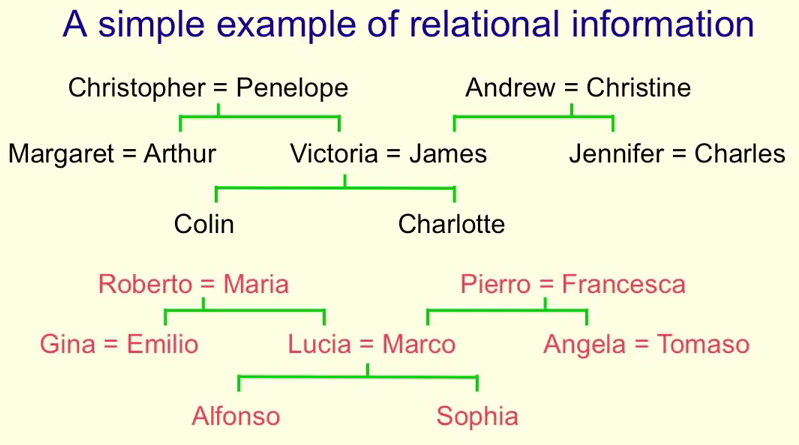
\includegraphics[scale=.5]{../Figuras/Hinton/ArbolGenealogico.png}
   \caption{Ejemplo de un árbol genealogico de familias nucleares.}
  \label{fig:arbolG}
  \end{figure}

En el árbol anterior se pueden apreciar que existen las siguientes 12 relaciones entre personas; hijo, hija, sobrino, sobrina, padre, madre, tío, tía, hermano, hermana, esposo, esposa. Y vamos a tener la siguientes proposiciones para denotarlas se la siguiente forma; 

\begin{itemize}
 \item (colin tiene-padre james)
 \item(colin tiene-madre victoria)
 \item(james tiene-esposa victoria)(colin tiene-padre james)
 \item(colin tiene-madre victoria)
 \item(james tiene-esposa victoria) 
\end{itemize}

La tarea objetivo: \textit{Que la red siguiente indique la segunda persona de la tercia, dados los valores en las dos primeras posiciones.} Si tenemos los valores [nombre entrada] [tiene-relación] [nombre salida], con los dos primeros datos nos debe dar el tercer dato.

El árbol familiar que se mostro arriba se puede ver como la red mostrada en la \fref{fig:redRelaciones}.
  \begin{figure}[h]
   \centering
   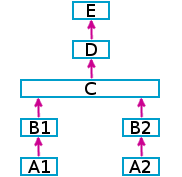
\includegraphics[scale=.5]{../Figuras/Hinton/RedRelaciones.png}
   \caption{Red de relaciones.}
  \label{fig:redRelaciones}
  \end{figure}

El diseño de la red es como se puede ver en la  \fref{RedHinton86}:

\begin{itemize}
 \item Capa uno:
 \begin{itemize}
  \item 24 neuronas de entrada (una para cada persona).
  \item 12 neuronas de entrada (una para cada relación).
 \end{itemize}
\item Capa dos:
 \begin{itemize}
  \item 6 neuronas conectadas con las 24 personas.
  \item 6 neuronas conectadas con las 12 relaciones.
 \end{itemize}
\item Capa tres:
 \begin{itemize}
  \item 12 neuronas conectadas a todas las neuronas en la capa 2.
 \end{itemize}
\item Capa cuatro:
 \begin{itemize}
  \item 6 neuronas conectadas a todas las neuronas en la capa 3.
 \end{itemize}
\item Capa cinco:
 \begin{itemize}
  \item 24 neuronas de salida, una para cada persona relacionada con la de entrada.
 \end{itemize}

\end{itemize}


Las datos de entrada son: 112 proposiciones, 100 utilizadas para entrenamiento, con 1500 iteraciones.

  \begin{figure}[h]
   \centering
   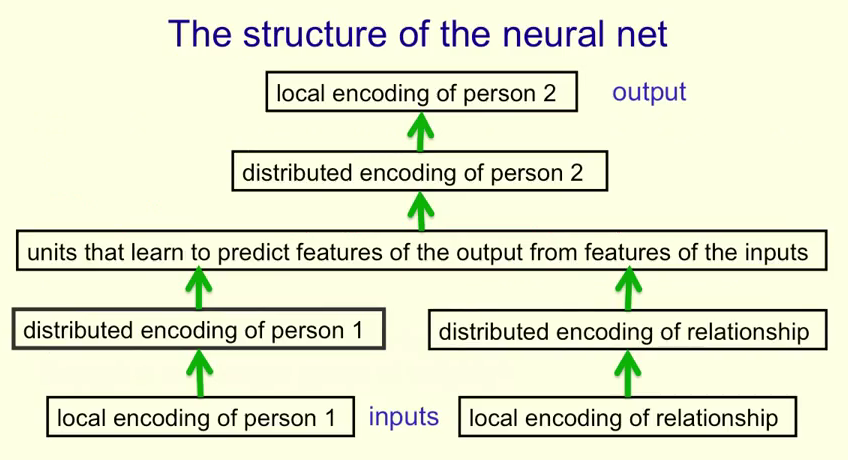
\includegraphics[scale=.5]{../Figuras/Hinton/RedHinton86.png}
   \caption{Estructura propuesta para la red neuronal de parentesco familiar.}
  \label{fig:RH86}
  \end{figure}

Las seis neuronas ocultas en el cuello de botella conectado a la entrada representa las características de las personas que
son útiles para predecir la salida, tales como, la rama del árbol genealógico al que pertenece.
La capa central aprende cómo las características predicen
otras características. Por ejemplo, la persona de entrada es de generación 3 y la relación requiere que la respuesta sea una generación más, entonces implica que la persona de salida es de la generación 2.

Ya con la estructura de la red definida podemos hacer el entrenamiento, primero con la alimentación hacia adelante, 

  \begin{figure}[h]
   \centering
   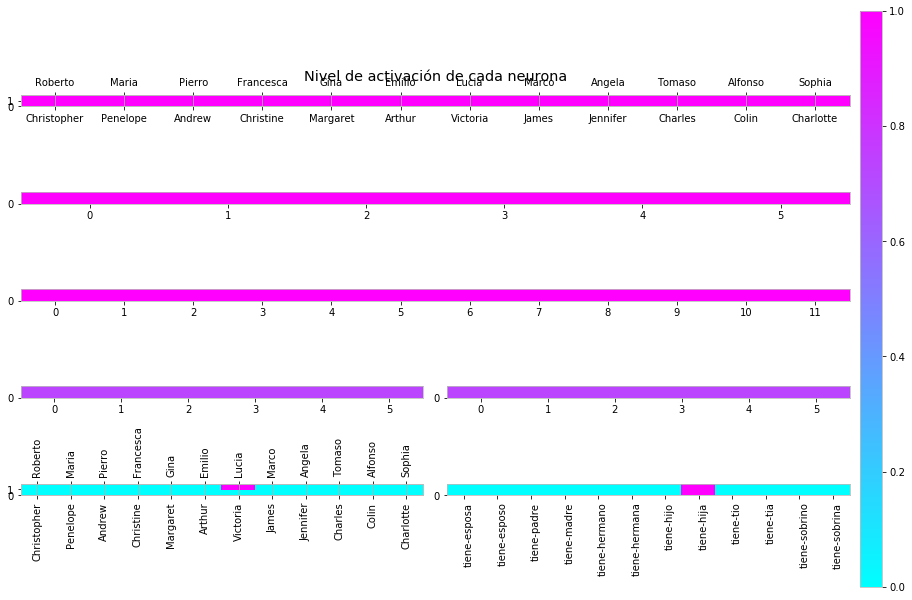
\includegraphics[scale=.5]{../Figuras/Hinton/r1.png}
   \caption{Primeras resoluciones.}
  \label{fig:r1}
  \end{figure}

    \begin{figure}[h]
   \centering
   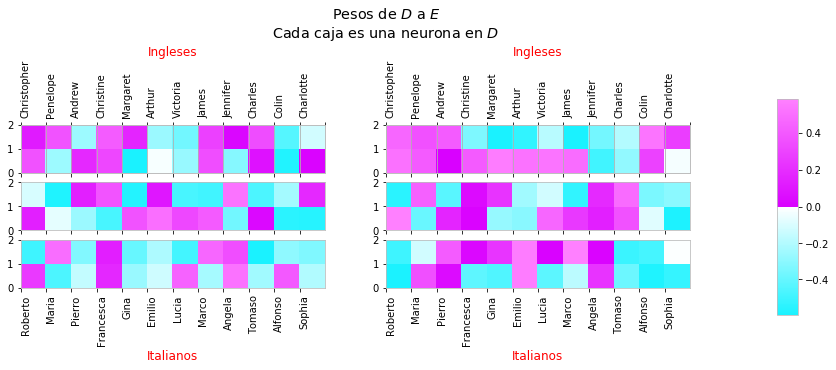
\includegraphics[scale=.5]{../Figuras/Hinton/r2.png}
   \caption{Resoluciones.}
  \label{fig:r2}
  \end{figure}

    \begin{figure}[h]
   \centering
   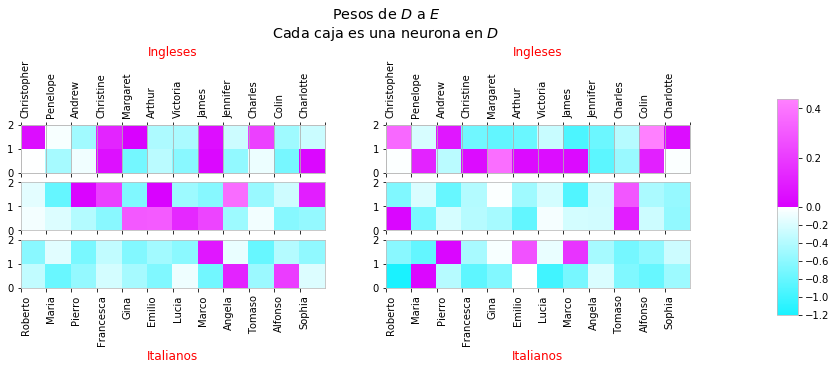
\includegraphics[scale=.5]{../Figuras/Hinton/r3.png}
   \caption{Resoluciones.}
  \label{fig:r3}
  \end{figure}
